
\newpage
\section{Unity ML-Agents}\label{appendix:mlagents}

\subsection{Visual Encoders}\label{appendix:visual-encoders}
todo 

\subsection{PPO Trainer: Hyperparameters}\label{appendix:ppo-trainer}

\begin{longtable}{@{} p{3.5cm} p{2.5cm} p{2.5cm} @{}} \toprule
\textbf{Hyperparemeter}       & \textbf{Default Value} & \textbf{Typical Range} \\ \midrule
visual encoder type         & simple    & - \\ 
normalize                   & false     & - \\
learning rate               & 3e-4      & 1e-5 - 1e-3 \\ 
learning rate schedule      & linear    & linear, constant \\ 
batch size                  &  1024     & 512 - 5120 \\
max steps                   &  500000   & 5e5 - 1e7 \\ 
buffer size                 & 10240     & 2048 - 409600 \\ 
time horizon                &  64       & 32 - 2048  \\
number of layers            &  2        & 1-3 \\
hidden units                &  128      & 32-512 \\
beta                        &  5.0e-3   & 1e-4 - 1e-2  \\
epsilon                     &  0.2      & 0.1 - 0.3  \\
lambda                      &  0.95     & 0.9 - 0.95  \\
number of epochs            & 3         & 3 - 10 \\ \bottomrule
% number of epochs                        & ROSTeat node is running. \\ \cmidrule{1-2} 
% Exceptions             & Image is not RGB \\ \bottomrule
\caption{Default hyperparameters in PPO trainer, taken from \cite{github-unity-mlagents-toolkit}} \label{tab:default-hyperparameters}
% \\
\end{longtable}

\newpage

\subsection{Class Model Diagram of C\# Implementation}

TODO insert C# model diagram.



\newpage
% \subsection{Example Training Configuration File}\label{appendix:ppo-trainer}
% \newpage
\begin{multicols}{2}
[
\subsection{Example Training Configuration File}\label{appendix:ppo-trainer}
% All human things are subject to decay. And when fate summons, Monarchs must obey.
]
\begin{minted}[
    gobble=4,
    frame=single,
    linenos
  ]{yaml}
    # config file: run63++100.yaml
    behaviors:
      Drone:
        trainer_type: ppo
        hyperparameters:
          batch_size: 1024
          buffer_size: 10240
          learning_rate: 0.0003
          beta: 0.01
          epsilon: 0.2
          lambd: 0.95
          num_epoch: 3
          learning_rate_schedule: linear
        network_settings:
          normalize: false
          hidden_units: 256
          num_layers: 2
          vis_encode_type: simple
          # no lstm
        reward_signals:
          extrinsic:
            gamma: 0.99
            strength: 1.0
          curiosity:
            gamma: 0.99
            strength: 0.02
            network_settings:
              hidden_units: 256
            learning_rate: 0.0003
        keep_checkpoints: 5
        max_steps: 20000000
        time_horizon: 64
        summary_freq: 30000
\end{minted}
\columnbreak

\begin{minted}[
    gobble=4,
    frame=single,
    % linenos
  ]{yaml}
    environment_parameters:
      # 0:base, 1:open, 2:fire, 3:forest
      EnvironmentType: 0 
      steuernModus: 1
      m_EnableVFX: 0
      m_EnableTrainDebuggingLogs: 0
      # base
      m_TrainMovingForward: 1
      m_TrainTargetSpeed: 1
      # octree
      leafNodeSize: 4
      m_AddOctreeObservations: 0
      m_TrainOctreeDiscovery: 0
      m_TrainLingerPolicy: 0
      m_AddPigeonObservations: 0
      # voxel
      m_TrainVoxelCollection: 1
      allowedToSeeVoxels: 1
      m_VoxelRewardStrength: 1
      NormalizeVoxelReward: 0 
      # enabled for all voxel-behaviors
      m_SpeedSensitivityToTargetsInFOV: 1
      # shortest
      m_AddShortestPathObservations: 0
      m_TrainShortestPath: 0
      # detector
      m_LoadDetector: 0
      m_AddDetectorObservations: 0
      m_TrainObjectDetectionMaximization: 0
      NormalizeDetectionsReward: 1
      # curiosity
      m_AddSemanticCuriosityObservations: 0
      m_TrainSemanticCuriosity: 0
      # entropy
      m_AddSemanticEntropyObservations: 0
      m_TrainSemanticEntropy: 0
\end{minted}

\end{multicols}

\subsection{In-depth Metrics}\label{appendix:indepth-metrics}
% The full list of in-depth metrics is listed below:
    \begin{multicols}{3}
\begin{itemize}
    \item name
    \item speed
    \item linger
    \item pigeon
    \item pathak
    \item constrained
    \item node\_size
    \item train\_octree\_discovery
    \item train\_voxel\_discovery
    \item voxel\_reward\_str
    \item voxel\_vision
    \item oracle
    \item train\_entropy
    \item sac
    \item n\_leafNodes
    \item n\_leafNodes\_y
    \item leafNodeVolume
    \item \%leafNodesExplored
    \item \%scanNodesExplored
    \item visual\_analysis %\_confirms\_best
    \item \%episode\_length
    \item avg\_total\_objects\_scanned
\end{itemize}
\end{multicols}


\begin{sidewaystable}
\subsection{Agent Definitions by Observations}\label{appendix:baselines}
 
    % \hspace{-\marginparsep}    
    % \hspace{-0.5\marginparwidth}
  
    \begin{longtable}{l|cccccccc|l}
    \cline{2-9}
     & \multicolumn{8}{c|}{Obs. per Baseline} &  \\ \hline
    \multicolumn{1}{|l|}{Baseline} & \multicolumn{1}{c|}{\begin{tabular}[c]{@{}c@{}}Octree \\ Obs.\end{tabular}} & \multicolumn{1}{c|}{\begin{tabular}[c]{@{}c@{}}Voxel \\ Vision\end{tabular}} & \multicolumn{1}{c|}{\begin{tabular}[c]{@{}c@{}}Pigeon\\ Obs.\end{tabular}} & \multicolumn{1}{l|}{\begin{tabular}[c]{@{}l@{}}Speed \\ Sensitivity \\ to FOV\end{tabular}} & \multicolumn{1}{c|}{\begin{tabular}[c]{@{}c@{}}Shortest \\ Path\\  Obs.\end{tabular}} & \multicolumn{1}{c|}{\begin{tabular}[c]{@{}c@{}}Detector \\ Obs.\end{tabular}} & \multicolumn{1}{c|}{\begin{tabular}[c]{@{}c@{}}Semantic \\ Curiosity \\ Obs.\end{tabular}} & \begin{tabular}[c]{@{}c@{}}Semantic \\ Entropy \\ Obs.\end{tabular} & \multicolumn{1}{l|}{Comment} \\ \hline
    
    \multicolumn{1}{|l|}{Random Walk} & \multicolumn{1}{c|}{} & \multicolumn{1}{c|}{} & \multicolumn{1}{c|}{} & \multicolumn{1}{c|}{} & \multicolumn{1}{c|}{} & \multicolumn{1}{c|}{} & \multicolumn{1}{c|}{} &  & \multicolumn{1}{l|}
    {Simple agent with obs: speed and position in 3D space.} \\ \hline
    
    \multicolumn{1}{|l|}{Octree Agent} & \multicolumn{1}{c|}{\emoji{x}} & \multicolumn{1}{c|}{} & \multicolumn{1}{c|}{\emoji{x}} & \multicolumn{1}{c|}{} & \multicolumn{1}{c|}{} & \multicolumn{1}{c|}{} & \multicolumn{1}{c|}{} &  & \multicolumn{1}{l|}
    {DA with discovered octree nodes count each timestep.} \\ \hline
    
    \multicolumn{1}{|l|}{Voxel (R\_VOX norm)}  & \multicolumn{1}{c|}{} & \multicolumn{1}{c|}{\emoji{x}} & \multicolumn{1}{c|}{} & \multicolumn{1}{c|}{\emoji{x}} & \multicolumn{1}{c|}{} & \multicolumn{1}{c|}{} & \multicolumn{1}{c|}{} &  & \multicolumn{1}{l|}{
    DA that observes voxels with a normalized reward.} \\ \hline
    
    \multicolumn{1}{|l|}{Voxel (R\_VOX str: 0.25)}  & \multicolumn{1}{c|}{} & \multicolumn{1}{c|}{\emoji{x}} & \multicolumn{1}{c|}{} & \multicolumn{1}{c|}{\emoji{x}} & \multicolumn{1}{c|}{} & \multicolumn{1}{c|}{} & \multicolumn{1}{c|}{} &  & \multicolumn{1}{l|}{
    DA that observes voxels with a reward strength of 25\%} \\ \hline
    
    \multicolumn{1}{|l|}{Voxel (R\_VOX str: 0.50)}   & \multicolumn{1}{c|}{} & \multicolumn{1}{c|}{\emoji{x}} & \multicolumn{1}{c|}{} & \multicolumn{1}{c|}{\emoji{x}} & \multicolumn{1}{c|}{} & \multicolumn{1}{c|}{} & \multicolumn{1}{c|}{} &  & \multicolumn{1}{l|}{
    DA that observes voxels with a reward strength of 50\%} \\ \hline
    
    \multicolumn{1}{|l|}{Voxel (R\_VOX str: 0.75)}  & \multicolumn{1}{c|}{} & \multicolumn{1}{c|}{\emoji{x}} & \multicolumn{1}{c|}{} & \multicolumn{1}{c|}{\emoji{x}} & \multicolumn{1}{c|}{} & \multicolumn{1}{c|}{} & \multicolumn{1}{c|}{} &  & \multicolumn{1}{l|}{
    DA that observes voxels with a reward strength of 75\%} \\ \hline
    
    \multicolumn{1}{|l|}{Voxel (R\_VOX str: 1.00)}   & \multicolumn{1}{c|}{} & \multicolumn{1}{c|}{\emoji{x}} & \multicolumn{1}{c|}{} & \multicolumn{1}{c|}{\emoji{x}} & \multicolumn{1}{c|}{} & \multicolumn{1}{c|}{} & \multicolumn{1}{c|}{} &  & \multicolumn{1}{l|}{
    DA that observes voxels with a reward strength of 100\%} \\ \hline
    
    \multicolumn{1}{|l|}{Shortest Path}  & \multicolumn{1}{c|}{} & \multicolumn{1}{c|}{} & \multicolumn{1}{c|}{} & \multicolumn{1}{c|}{\emoji{x}} & \multicolumn{1}{c|}{\emoji{x}} & \multicolumn{1}{c|}{} & \multicolumn{1}{c|}{} &  & \multicolumn{1}{l|}{
    DA with walk angle and look angle to target.} \\ \hline

    \multicolumn{1}{|l|}{Shortest Path + Vision}  & \multicolumn{1}{c|}{} & \multicolumn{1}{c|}{\emoji{x}} & \multicolumn{1}{c|}{} & \multicolumn{1}{c|}{\emoji{x}} & \multicolumn{1}{c|}{} & \multicolumn{1}{c|}{} & \multicolumn{1}{c|}{} &  & \multicolumn{1}{l|}{
    DA with voxel vision.} \\ \hline
    
    \multicolumn{1}{|l|}{Object Detection} & \multicolumn{1}{c|}{} & \multicolumn{1}{c|}{} & \multicolumn{1}{c|}{} & \multicolumn{1}{c|}{\emoji{x}} & \multicolumn{1}{c|}{} & \multicolumn{1}{c|}{\emoji{x}} & \multicolumn{1}{c|}{} &  & \multicolumn{1}{l|}{
    Simple agent with input from object detector.} \\ \hline

    \multicolumn{1}{|l|}{Object Detection + pure} & \multicolumn{1}{c|}{} & \multicolumn{1}{c|}{} & \multicolumn{1}{c|}{} & \multicolumn{1}{c|}{\emoji{x}} & \multicolumn{1}{c|}{} & \multicolumn{1}{c|}{} & \multicolumn{1}{c|}{} &  & \multicolumn{1}{l|}{
    Simple agent without speed constraint.} \\ \hline
    
    \multicolumn{1}{|l|}{Semantic Curiosity} & \multicolumn{1}{c|}{} & \multicolumn{1}{c|}{} & \multicolumn{1}{c|}{} & \multicolumn{1}{c|}{\emoji{x}} & \multicolumn{1}{c|}{} & \multicolumn{1}{c|}{} & \multicolumn{1}{c|}{\emoji{x}} &  & \multicolumn{1}{l|}{
    DA with rationalized class density each timestep.} \\ \hline
    
    \multicolumn{1}{|l|}{Semantic Entropy}& \multicolumn{1}{c|}{} & \multicolumn{1}{c|}{} & \multicolumn{1}{c|}{} & \multicolumn{1}{c|}{\emoji{x}} & \multicolumn{1}{c|}{} & \multicolumn{1}{c|}{} & \multicolumn{1}{c|}{} &  & \multicolumn{1}{l|}{
    DA with lingering penalty strength present reduction.} \\ \hline
    
    \multicolumn{1}{|l|}{Explorer (R\_VOX str: 0.5)}  & \multicolumn{1}{c|}{\emoji{x}} & \multicolumn{1}{c|}{\emoji{x}} & \multicolumn{1}{c|}{\emoji{x}} & \multicolumn{1}{c|}{\emoji{x}} & \multicolumn{1}{c|}{} & \multicolumn{1}{c|}{} & \multicolumn{1}{c|}{} & \emoji{x} & \multicolumn{1}{l|}
    {DA as above. Voxel reward strength of 50\%} \\ \hline
    
    \multicolumn{1}{|l|}{Explorer (R\_VOX str: 1.0)} & \multicolumn{1}{c|}{\emoji{x}} & \multicolumn{1}{c|}{\emoji{x}} & \multicolumn{1}{c|}{\emoji{x}} & \multicolumn{1}{c|}{\emoji{x}} & \multicolumn{1}{c|}{} & \multicolumn{1}{c|}{} & \multicolumn{1}{c|}{} & \emoji{x} & \multicolumn{1}{l|}
    {DA as above. Voxel reward strength of 100\%} \\ \hline
    
    \caption{Diverse agent behavior variants and the observations they receive. "DA" stands for Derived Agent. All agents observe their own information, such as 3D position, orientation, etc.}
    \label{appendix:baselines_observations}
    
    \end{longtable}%

        % \usepackage{graphicx}
       
\end{sidewaystable}


\begin{sidewaystable}
\subsection{Agent Definitions by Rewards}
 
    % \hspace{-\marginparsep}    
    % \hspace{-0.5\marginparwidth}
  
    \begin{longtable}{l|ccccccc|l}
    \cline{2-8}
             & \multicolumn{7}{c|}{Trained Functions} &  \\ \hline
            %  \multicolumn{1}{c|}{\begin{tabular}[c]{@{}c@{}} Moving \\ Forward\end{tabular}}
            \multicolumn{1}{|l|}{Baseline}  & \multicolumn{1}{c|}{\begin{tabular}[c]{@{}c@{}} Speed\end{tabular}} & \multicolumn{1}{c|}{\begin{tabular}[c]{@{}c@{}}  Octree \\ Nodes\\  Discovery\end{tabular}} & \multicolumn{1}{c|}{\begin{tabular}[c]{@{}c@{}} Voxel \\ Discovery\end{tabular}} & \multicolumn{1}{c|}{\begin{tabular}[c]{@{}c@{}} Shortest \\ Path\end{tabular}} & \multicolumn{1}{c|}{\begin{tabular}[c]{@{}c@{}} Object \\ Detection\end{tabular}} & \multicolumn{1}{c|}{\begin{tabular}[c]{@{}c@{}} Semantic \\ Curiosity\end{tabular}} & \begin{tabular}[c]{@{}c@{}} Semantic \\ Entropy\end{tabular} & \multicolumn{1}{l|}{Comment} \\ \hline
            
            \multicolumn{1}{|l|}{Random Walk}  & \multicolumn{1}{c|}{\emoji{x}} & \multicolumn{1}{c|}{} & \multicolumn{1}{c|}{} & \multicolumn{1}{c|}{} & \multicolumn{1}{c|}{} & \multicolumn{1}{c|}{} &  & \multicolumn{1}{l|}
            {Simple that moves at a minimum target speed.} \\ \hline
            
            \multicolumn{1}{|l|}{Octree Agent} & \multicolumn{1}{c|}{\emoji{x}} & \multicolumn{1}{c|}{\emoji{x}} & \multicolumn{1}{c|}{} & \multicolumn{1}{c|}{} & \multicolumn{1}{c|}{} & \multicolumn{1}{c|}{} &  & \multicolumn{1}{l|}
            {DA that explores new (octree) locations.} \\ \hline
            
            \multicolumn{1}{|l|}{Voxel (R\_VOX norm)} & \multicolumn{1}{c|}{\emoji{x}} & \multicolumn{1}{c|}{} & \multicolumn{1}{c|}{\emoji{x}} & \multicolumn{1}{c|}{} & \multicolumn{1}{c|}{} & \multicolumn{1}{c|}{} &  & \multicolumn{1}{l|}
            {""                               ""} \\ \hline
            
            \multicolumn{1}{|l|}{Voxel (R\_VOX str: 0.25)} & \multicolumn{1}{c|}{\emoji{x}} & \multicolumn{1}{c|}{} & \multicolumn{1}{c|}{\emoji{x}} & \multicolumn{1}{c|}{} & \multicolumn{1}{c|}{} & \multicolumn{1}{c|}{} &  & \multicolumn{1}{l|}
            {""                               ""} \\ \hline
        
            \multicolumn{1}{|l|}{Voxel (R\_VOX str: 0.50)} & \multicolumn{1}{c|}{\emoji{x}} & \multicolumn{1}{c|}{} & \multicolumn{1}{c|}{\emoji{x}} & \multicolumn{1}{c|}{} & \multicolumn{1}{c|}{} & \multicolumn{1}{c|}{} &  & \multicolumn{1}{l|}
            {""                               ""} \\ \hline
        
            \multicolumn{1}{|l|}{Voxel (R\_VOX str: 0.75)}  & \multicolumn{1}{c|}{\emoji{x}} & \multicolumn{1}{c|}{} & \multicolumn{1}{c|}{\emoji{x}} & \multicolumn{1}{c|}{} & \multicolumn{1}{c|}{} & \multicolumn{1}{c|}{} &  & \multicolumn{1}{l|}
            {""                               ""} \\ \hline
        
            \multicolumn{1}{|l|}{Voxel (R\_VOX str: 1.00)}  & \multicolumn{1}{c|}{\emoji{x}} & \multicolumn{1}{c|}{} & \multicolumn{1}{c|}{\emoji{x}} & \multicolumn{1}{c|}{} & \multicolumn{1}{c|}{} & \multicolumn{1}{c|}{} &  & \multicolumn{1}{l|}
            {""                               ""} \\ \hline
        
            \multicolumn{1}{|l|}{Shortest Path}  & \multicolumn{1}{c|}{\emoji{x}} & \multicolumn{1}{c|}{} & \multicolumn{1}{c|}{\emoji{x}} & \multicolumn{1}{c|}{\emoji{x}} & \multicolumn{1}{c|}{} & \multicolumn{1}{c|}{} &  & \multicolumn{1}{l|}
            {DA that learns to move to the closest target.} \\ \hline
        
            
            \multicolumn{1}{|l|}{Shortest Path + Vision} & \multicolumn{1}{c|}{\emoji{x}} & \multicolumn{1}{c|}{} & \multicolumn{1}{c|}{\emoji{x}} & \multicolumn{1}{c|}{\emoji{x}} & \multicolumn{1}{c|}{} & \multicolumn{1}{c|}{} &  & \multicolumn{1}{l|}
            {DA with voxel vision.} \\ \hline
        
            
            \multicolumn{1}{|l|}{Object Detection} & \multicolumn{1}{c|}{\emoji{x}} & \multicolumn{1}{c|}{} & \multicolumn{1}{c|}{\emoji{x}} & \multicolumn{1}{c|}{} & \multicolumn{1}{c|}{\emoji{x}} & \multicolumn{1}{c|}{} &  & \multicolumn{1}{l|}
            {DA that maximizes object detections.} \\ \hline
            
            \multicolumn{1}{|l|}{Object Detection + pure} & \multicolumn{1}{c|}{} & \multicolumn{1}{c|}{} & \multicolumn{1}{c|}{\emoji{x}} & \multicolumn{1}{c|}{} & \multicolumn{1}{c|}{\emoji{x}} & \multicolumn{1}{c|}{} &  & \multicolumn{1}{l|}
            {DA with no minimum speed penalty.} \\ \hline
        % . Found voxels provide a normalized reward.}
            
            \multicolumn{1}{|l|}{Semantic Curiosity}  & \multicolumn{1}{c|}{\emoji{x}} & \multicolumn{1}{c|}{} & \multicolumn{1}{c|}{\emoji{x}} & \multicolumn{1}{c|}{} & \multicolumn{1}{c|}{} & \multicolumn{1}{c|}{\emoji{x}} &  & \multicolumn{1}{l|}
            {DA that maximizes the temporal class density.} \\ \hline
            
            \multicolumn{1}{|l|}{Ultron (Semantic Entropy)} & \multicolumn{1}{c|}{\emoji{x}} & \multicolumn{1}{c|}{} & \multicolumn{1}{c|}{\emoji{x}} & \multicolumn{1}{c|}{} & \multicolumn{1}{c|}{} & \multicolumn{1}{c|}{} & \emoji{x} & \multicolumn{1}{l|}
            {Voxel-DA with a lingering penalty regulator.} \\ \hline
            
            \multicolumn{1}{|l|}{Explorer (R\_VOX str: 0.5)} & \multicolumn{1}{c|}{\emoji{x}} & \multicolumn{1}{c|}{\emoji{x}} & \multicolumn{1}{c|}{\emoji{x}} & \multicolumn{1}{c|}{} & \multicolumn{1}{c|}{} & \multicolumn{1}{c|}{} & \emoji{x} & \multicolumn{1}{l|}
            {Explorer DA for voxels and octrees.} \\ \hline
            
            \multicolumn{1}{|l|}{Explorer (R\_VOX str: 1.0)}  & \multicolumn{1}{c|}{\emoji{x}} & \multicolumn{1}{c|}{\emoji{x}} & \multicolumn{1}{c|}{\emoji{x}} & \multicolumn{1}{c|}{} & \multicolumn{1}{c|}{} & \multicolumn{1}{c|}{} & \emoji{x} & \multicolumn{1}{l|}
            {Explorer DA for voxels and octrees.} \\ \hline
            
    
    \caption{Diverse agent behavior variants and the rewards they receive. "DA" stands for Derived Agent.}
    \label{appendix:baselines_observations}
    
    \end{longtable}%

        % \usepackage{graphicx}
       
\end{sidewaystable}

% \begin{sidewaystable}
 
%  \begin{table}[]
%         \hspace{-\marginparsep}    
%         \hspace{-0.5\marginparwidth}
%         \resizebox{1.65\textwidth}{!}{%
%             \begin{tabular}{l|cccccccc|l}
%             \cline{2-9}
%              & \multicolumn{8}{c|}{Rewards per Baseline} &  \\ \hline
%             \multicolumn{1}{|l|}{Baseline} & \multicolumn{1}{c|}{\begin{tabular}[c]{@{}c@{}}Train Moving \\ Forward\end{tabular}} & \multicolumn{1}{c|}{\begin{tabular}[c]{@{}c@{}} Speed\end{tabular}} & \multicolumn{1}{c|}{\begin{tabular}[c]{@{}c@{}}Train Octree \\ Nodes Discovery\end{tabular}} & \multicolumn{1}{c|}{\begin{tabular}[c]{@{}c@{}}Train Voxel \\ Discovery\end{tabular}} & \multicolumn{1}{c|}{\begin{tabular}[c]{@{}c@{}}Train Shortest \\ Path\end{tabular}} & \multicolumn{1}{c|}{\begin{tabular}[c]{@{}c@{}}Train Object \\ Detection\end{tabular}} & \multicolumn{1}{c|}{\begin{tabular}[c]{@{}c@{}}Train Semantic \\ Curiosity\end{tabular}} & \begin{tabular}[c]{@{}c@{}}Train Semantic \\ Entropy\end{tabular} & \multicolumn{1}{l|}{Comment} \\ \hline
%             \multicolumn{1}{|l|}{Random Walk} & \multicolumn{1}{c|}{\emoji{x}} & \multicolumn{1}{c|}{\emoji{x}} & \multicolumn{1}{c|}{} & \multicolumn{1}{c|}{} & \multicolumn{1}{c|}{} & \multicolumn{1}{c|}{} & \multicolumn{1}{c|}{} &  & \multicolumn{1}{l|}{Simple agent that learns to move to reach a minimum target speed.} \\ \hline
%             \multicolumn{1}{|l|}{Octree Agent} & \multicolumn{1}{c|}{\emoji{x}} & \multicolumn{1}{c|}{\emoji{x}} & \multicolumn{1}{c|}{\emoji{x}} & \multicolumn{1}{c|}{} & \multicolumn{1}{c|}{} & \multicolumn{1}{c|}{} & \multicolumn{1}{c|}{} &  & \multicolumn{1}{l|}{DA that learns how to discover octree nodes while it moves.} \\ \hline
%             \multicolumn{1}{|l|}{Voxel (R\_VOX norm)} & \multicolumn{1}{c|}{\emoji{x}} & \multicolumn{1}{c|}{\emoji{x}} & \multicolumn{1}{c|}{} & \multicolumn{1}{c|}{\emoji{x}} & \multicolumn{1}{c|}{} & \multicolumn{1}{c|}{} & \multicolumn{1}{c|}{} &  & \multicolumn{1}{l|}{""                                                                                             ""} \\ \hline
%             \multicolumn{1}{|l|}{Voxel (R\_VOX str: 0.25)} & \multicolumn{1}{c|}{\emoji{x}} & \multicolumn{1}{c|}{\emoji{x}} & \multicolumn{1}{c|}{} & \multicolumn{1}{c|}{\emoji{x}} & \multicolumn{1}{c|}{} & \multicolumn{1}{c|}{} & \multicolumn{1}{c|}{} &  & \multicolumn{1}{l|}{""                                                                                             ""} \\ \hline
%             \multicolumn{1}{|l|}{Voxel (R\_VOX str: 0.50)} & \multicolumn{1}{c|}{\emoji{x}} & \multicolumn{1}{c|}{\emoji{x}} & \multicolumn{1}{c|}{} & \multicolumn{1}{c|}{\emoji{x}} & \multicolumn{1}{c|}{} & \multicolumn{1}{c|}{} & \multicolumn{1}{c|}{} &  & \multicolumn{1}{l|}{""                                                                                             ""} \\ \hline
%             \multicolumn{1}{|l|}{Voxel (R\_VOX str: 0.75)} & \multicolumn{1}{c|}{\emoji{x}} & \multicolumn{1}{c|}{\emoji{x}} & \multicolumn{1}{c|}{} & \multicolumn{1}{c|}{\emoji{x}} & \multicolumn{1}{c|}{} & \multicolumn{1}{c|}{} & \multicolumn{1}{c|}{} &  & \multicolumn{1}{l|}{""                                                                                             ""} \\ \hline
%             \multicolumn{1}{|l|}{Voxel (R\_VOX str: 1.00)} & \multicolumn{1}{c|}{\emoji{x}} & \multicolumn{1}{c|}{\emoji{x}} & \multicolumn{1}{c|}{} & \multicolumn{1}{c|}{\emoji{x}} & \multicolumn{1}{c|}{} & \multicolumn{1}{c|}{} & \multicolumn{1}{c|}{} &  & \multicolumn{1}{l|}{""                                                                                             ""} \\ \hline
%             \multicolumn{1}{|l|}{Shortest Path + Vision} & \multicolumn{1}{c|}{\emoji{x}} & \multicolumn{1}{c|}{\emoji{x}} & \multicolumn{1}{c|}{} & \multicolumn{1}{c|}{\emoji{x}} & \multicolumn{1}{c|}{\emoji{x}} & \multicolumn{1}{c|}{} & \multicolumn{1}{c|}{} &  & \multicolumn{1}{l|}{DA that learns to move directly to the next target. Found voxels provide a normalized reward.} \\ \hline
%             \multicolumn{1}{|l|}{Shortest Path} & \multicolumn{1}{c|}{\emoji{x}} & \multicolumn{1}{c|}{\emoji{x}} & \multicolumn{1}{c|}{} & \multicolumn{1}{c|}{\emoji{x}} & \multicolumn{1}{c|}{\emoji{x}} & \multicolumn{1}{c|}{} & \multicolumn{1}{c|}{} &  & \multicolumn{1}{l|}{DA that learns to move directly to the next target. Found voxels provide a normalized reward.} \\ \hline
%             \multicolumn{1}{|l|}{Object Detection + pure} & \multicolumn{1}{c|}{\emoji{x}} & \multicolumn{1}{c|}{} & \multicolumn{1}{c|}{} & \multicolumn{1}{c|}{\emoji{x}} & \multicolumn{1}{c|}{} & \multicolumn{1}{c|}{\emoji{x}} & \multicolumn{1}{c|}{} &  & \multicolumn{1}{l|}{DA that learns how to maximize object detections. Found voxels provide a normalized reward.} \\ \hline
%             \multicolumn{1}{|l|}{Object Detection} & \multicolumn{1}{c|}{\emoji{x}} & \multicolumn{1}{c|}{\emoji{x}} & \multicolumn{1}{c|}{} & \multicolumn{1}{c|}{\emoji{x}} & \multicolumn{1}{c|}{} & \multicolumn{1}{c|}{\emoji{x}} & \multicolumn{1}{c|}{} &  & \multicolumn{1}{l|}{DA that learns how to maximize object detections. Found voxels provide a normalized reward.} \\ \hline
%             % \multicolumn{1}{|l|}{Semantic Curiosity} & \multicolumn{1}{c|}{\emoji{x}} & \multicolumn{1}{c|}{\emoji{x}} & \multicolumn{1}{c|}{} & \multicolumn{1}{c|}{\emoji{x}} & \multicolumn{1}{c|}{} & \multicolumn{1}{c|}{} & \multicolumn{1}{c|}{\emoji{x}} &  & \multicolumn{1}{l|}{DA that learns how to maximize the temporal class density.} \\ \hline
%             % \multicolumn{1}{|l|}{Ultron (Semantic Entropy)} & \multicolumn{1}{c|}{\emoji{x}} & \multicolumn{1}{c|}{\emoji{x}} & \multicolumn{1}{c|}{} & \multicolumn{1}{c|}{\emoji{x}} & \multicolumn{1}{c|}{} & \multicolumn{1}{c|}{} & \multicolumn{1}{c|}{} & \emoji{x} & \multicolumn{1}{l|}{DA that learns how to discover octree nodes and scan voxels. Benefits from a lingering penalty strength regulator.} \\ \hline
%             % \multicolumn{1}{|l|}{Ultron (R\_VOX str: 0.5)} & \multicolumn{1}{c|}{\emoji{x}} & \multicolumn{1}{c|}{\emoji{x}} & \multicolumn{1}{c|}{\emoji{x}} & \multicolumn{1}{c|}{\emoji{x}} & \multicolumn{1}{c|}{} & \multicolumn{1}{c|}{} & \multicolumn{1}{c|}{} & \emoji{x} & \multicolumn{1}{l|}{DA as above. Voxel reward strength of 50\%} \\ \hline
%             % \multicolumn{1}{|l|}{Ultron (R\_VOX str: 1.0)} & \multicolumn{1}{c|}{\emoji{x}} & \multicolumn{1}{c|}{\emoji{x}} & \multicolumn{1}{c|}{\emoji{x}} & \multicolumn{1}{c|}{\emoji{x}} & \multicolumn{1}{c|}{} & \multicolumn{1}{c|}{} & \multicolumn{1}{c|}{} & \emoji{x} & \multicolumn{1}{l|}{DA as above. Voxel reward strength of 100\%} \\ \hline
%             \end{tabular}%
%         }
%         \caption{Diverse agent behavior variants and the rewards they receive.}
%         \label{appendix:baselines_rewards}
%         \end{table}
        
% \end{sidewaystable}


\begin{sidewaystable}
\subsection{Voxel-focused Agents}\label{appendix:RQ1-results-noknowledgeofvoxels}

\begin{longtable}{|l|c|c|c|c|c|}                            \hline
    % \multicolumn{3}{|l|}{\textbf{Voxel-Curiosity}}              \\\hline
    \thead{Method}            
    & \thead{Episode Length}                
    & \thead{Average Total \\ Objects Scanned}   
    & \thead{Modified \\ F1-score} 
    & \thead{Octree \\ Leaf Nodes Visited} 
    & \thead{Walk Error} 
    % & \thead{Total Detections Count} 
    \\ \hline

shortest-path+vision-nospeed & 88 & {\cellcolor[HTML]{EBF2F0}} \color[HTML]{000000} 0.04 & {\cellcolor[HTML]{EBF2F0}} \color[HTML]{000000} 0.01 & {\cellcolor[HTML]{EBF2F0}} \color[HTML]{000000} 0.06 & 	{\cellcolor[HTML]{55AA99}} \color[HTML]{F1F1F1} 0.20 \\ \hline
shortest-path+vision & 94 & {\cellcolor[HTML]{EBF2F0}} \color[HTML]{000000} 0.05 & {\cellcolor[HTML]{EBF2F0}} \color[HTML]{000000} 0.02 & {\cellcolor[HTML]{EBF2F0}} \color[HTML]{000000} 0.15 & 	{\cellcolor[HTML]{C8E1DC}} \color[HTML]{000000} 0.42 \\ \hline
shortest-path & 97 & {\cellcolor[HTML]{EBF2F0}} \color[HTML]{000000} 0.06 & {\cellcolor[HTML]{EBF2F0}} \color[HTML]{000000} 0.02 & {\cellcolor[HTML]{EBF2F0}} \color[HTML]{000000} 0.12 & 	{\cellcolor[HTML]{CFE5E0}} \color[HTML]{000000} 0.44 \\ \hline
semantic-curiosity & 99 & {\cellcolor[HTML]{EBF2F0}} \color[HTML]{000000} 0.07 & {\cellcolor[HTML]{EBF2F0}} \color[HTML]{000000} 0.02 & {\cellcolor[HTML]{EBF2F0}} \color[HTML]{000000} 0.10 & 	{\cellcolor[HTML]{D6E8E4}} \color[HTML]{000000} 0.45 \\ \hline
semantic-entropy & 40 & {\cellcolor[HTML]{EBF2F0}} \color[HTML]{000000} 0.13 & {\cellcolor[HTML]{EBF2F0}} \color[HTML]{000000} 0.04 & {\cellcolor[HTML]{EBF2F0}} \color[HTML]{000000} 0.11 & 	{\cellcolor[HTML]{EBF2F0}} \color[HTML]{000000} 0.49 \\ \hline
voxel & 89 & {\cellcolor[HTML]{D8E9E5}} \color[HTML]{000000} 0.40 & {\cellcolor[HTML]{EBF2F0}} \color[HTML]{000000} 0.10 & {\cellcolor[HTML]{E0EDEA}} \color[HTML]{000000} 0.22 & 	{\cellcolor[HTML]{E4EFEC}} \color[HTML]{000000} 0.48 \\ \hline
object-detector & 97 & {\cellcolor[HTML]{D9E9E6}} \color[HTML]{000000} 0.39 & {\cellcolor[HTML]{EBF2F0}} \color[HTML]{000000} 0.12 & {\cellcolor[HTML]{D1E6E1}} \color[HTML]{000000} 0.30 & 	{\cellcolor[HTML]{E2EEEB}} \color[HTML]{000000} 0.47 \\ \hline
blind-agent-voxel & 99 & {\cellcolor[HTML]{DDEBE8}} \color[HTML]{000000} 0.34 & {\cellcolor[HTML]{EBF2F0}} \color[HTML]{000000} 0.13 & {\cellcolor[HTML]{A3CFC6}} \color[HTML]{000000} 0.56 & 	{\cellcolor[HTML]{DBEBE7}} \color[HTML]{000000} 0.46 \\ \hline
voxel++100-nospeed-oracle-4 & 99 & {\cellcolor[HTML]{79BBAE}} \color[HTML]{000000} 1.64 & {\cellcolor[HTML]{EBF2F0}} \color[HTML]{000000} 0.13 & {\cellcolor[HTML]{EBF2F0}} \color[HTML]{000000} 0.15 & 	{\cellcolor[HTML]{B6D8D1}} \color[HTML]{000000} 0.39 \\ \hline
voxel++100-nospeed-nolinger-oracle-8 & 99 & {\cellcolor[HTML]{6EB6A7}} \color[HTML]{F1F1F1} 1.77 & {\cellcolor[HTML]{EBF2F0}} \color[HTML]{000000} 0.13 & {\cellcolor[HTML]{EBF2F0}} \color[HTML]{000000} 0.15 & 	{\cellcolor[HTML]{C3DFD9}} \color[HTML]{000000} 0.41 \\ \hline
blind-agent-voxel-constrained & 100 & {\cellcolor[HTML]{DEECE9}} \color[HTML]{000000} 0.33 & {\cellcolor[HTML]{EBF2F0}} \color[HTML]{000000} 0.13 & {\cellcolor[HTML]{7BBCAF}} \color[HTML]{000000} 0.79 & 	{\cellcolor[HTML]{E2EEEB}} \color[HTML]{000000} 0.47 \\ \hline
voxel++100 & 96 & {\cellcolor[HTML]{BCDCD5}} \color[HTML]{000000} 0.77 & {\cellcolor[HTML]{EBF2F0}} \color[HTML]{000000} 0.13 & {\cellcolor[HTML]{E3EEEC}} \color[HTML]{000000} 0.20 & 	{\cellcolor[HTML]{DEECE8}} \color[HTML]{000000} 0.47 \\ \hline
voxel++100-nospeed-nolinger-oracle & 95 & {\cellcolor[HTML]{90C6BB}} \color[HTML]{000000} 1.33 & {\cellcolor[HTML]{EBF2F0}} \color[HTML]{000000} 0.14 & {\cellcolor[HTML]{E7F0EE}} \color[HTML]{000000} 0.18 & 	{\cellcolor[HTML]{CBE3DE}} \color[HTML]{000000} 0.43 \\ \hline
voxel++100-nospeed-nolinger-pigeon-oracle-8 & 97 & {\cellcolor[HTML]{93C8BD}} \color[HTML]{000000} 1.30 & {\cellcolor[HTML]{EBF2F0}} \color[HTML]{000000} 0.14 & {\cellcolor[HTML]{E7F0EE}} \color[HTML]{000000} 0.18 & 	{\cellcolor[HTML]{CCE3DF}} \color[HTML]{000000} 0.43 \\ \hline
voxel++050 & 71 & {\cellcolor[HTML]{A6D1C8}} \color[HTML]{000000} 1.05 & {\cellcolor[HTML]{EBF2F0}} \color[HTML]{000000} 0.14 & {\cellcolor[HTML]{E3EFEC}} \color[HTML]{000000} 0.20 & 	{\cellcolor[HTML]{E6F0ED}} \color[HTML]{000000} 0.48 \\ \hline
object-detector-pure & 93 & {\cellcolor[HTML]{A9D2CA}} \color[HTML]{000000} 1.01 & {\cellcolor[HTML]{EBF2F0}} \color[HTML]{000000} 0.14 & {\cellcolor[HTML]{E3EEEC}} \color[HTML]{000000} 0.20 & 	{\cellcolor[HTML]{E1EDEA}} \color[HTML]{000000} 0.47 \\ \hline
voxel++075 & 98 & {\cellcolor[HTML]{ADD4CC}} \color[HTML]{000000} 0.96 & {\cellcolor[HTML]{EBF2F0}} \color[HTML]{000000} 0.14 & {\cellcolor[HTML]{E2EEEB}} \color[HTML]{000000} 0.21 & 	{\cellcolor[HTML]{DFECE9}} \color[HTML]{000000} 0.47 \\ \hline
object-detector-pure-vision & 99 & {\cellcolor[HTML]{80BFB2}} \color[HTML]{000000} 1.54 & {\cellcolor[HTML]{EBF2F0}} \color[HTML]{000000} 0.15 & {\cellcolor[HTML]{E6F0EE}} \color[HTML]{000000} 0.18 & 	{\cellcolor[HTML]{D9EAE6}} \color[HTML]{000000} 0.46 \\ \hline
voxel-entropy++100-oracle & 96 & {\cellcolor[HTML]{95C9BE}} \color[HTML]{000000} 1.27 & {\cellcolor[HTML]{E8F1EF}} \color[HTML]{000000} 0.16 & {\cellcolor[HTML]{E0EDEA}} \color[HTML]{000000} 0.22 & 	{\cellcolor[HTML]{DEECE9}} \color[HTML]{000000} 0.47 \\ \hline
voxel-entropy++100 & 89 & {\cellcolor[HTML]{A3D0C7}} \color[HTML]{000000} 1.08 & {\cellcolor[HTML]{E7F0EE}} \color[HTML]{000000} 0.16 & {\cellcolor[HTML]{DCEBE8}} \color[HTML]{000000} 0.24 & 	{\cellcolor[HTML]{E5EFED}} \color[HTML]{000000} 0.48 \\ \hline
voxel-entropy++100-oracle-nospeed & 98 & {\cellcolor[HTML]{7CBDB0}} \color[HTML]{000000} 1.59 & {\cellcolor[HTML]{E3EEEC}} \color[HTML]{000000} 0.17 & {\cellcolor[HTML]{DFEDE9}} \color[HTML]{000000} 0.22 & 	{\cellcolor[HTML]{D1E5E1}} \color[HTML]{000000} 0.44 \\ \hline
voxel-entropy++050 & 98 & {\cellcolor[HTML]{A0CEC4}} \color[HTML]{000000} 1.13 & {\cellcolor[HTML]{DFEDE9}} \color[HTML]{000000} 0.18 & {\cellcolor[HTML]{D8E9E5}} \color[HTML]{000000} 0.26 & 	{\cellcolor[HTML]{DEECE9}} \color[HTML]{000000} 0.47 \\ \hline
voxel++100-nospeed & 98 & {\cellcolor[HTML]{82C0B3}} \color[HTML]{000000} 1.52 & {\cellcolor[HTML]{D9EAE6}} \color[HTML]{000000} 0.19 & {\cellcolor[HTML]{D9EAE6}} \color[HTML]{000000} 0.26 & 	{\cellcolor[HTML]{DCEBE8}} \color[HTML]{000000} 0.46 \\ \hline
voxel++100-nospeed-oracle-8 & 94 & {\cellcolor[HTML]{CCE3DE}} \color[HTML]{000000} 0.56 & {\cellcolor[HTML]{D8E9E5}} \color[HTML]{000000} 0.19 & {\cellcolor[HTML]{8FC6BB}} \color[HTML]{000000} 0.67 & 	{\cellcolor[HTML]{DFEDE9}} \color[HTML]{000000} 0.47 \\ \hline
voxel++100-nospeed-nolinger & 97 & {\cellcolor[HTML]{71B8A9}} \color[HTML]{F1F1F1} 1.73 & {\cellcolor[HTML]{D7E9E5}} \color[HTML]{000000} 0.19 & {\cellcolor[HTML]{DAEAE6}} \color[HTML]{000000} 0.25 & 	{\cellcolor[HTML]{DFEDE9}} \color[HTML]{000000} 0.47 \\ \hline
voxel++025 & 94 & {\cellcolor[HTML]{7EBEB1}} \color[HTML]{000000} 1.56 & {\cellcolor[HTML]{D2E6E2}} \color[HTML]{000000} 0.20 & {\cellcolor[HTML]{D5E7E3}} \color[HTML]{000000} 0.28 & 	{\cellcolor[HTML]{DBEAE7}} \color[HTML]{000000} 0.46 \\ \hline
voxel-entropy++100-nospeed & 96 & {\cellcolor[HTML]{55AA99}} \color[HTML]{F1F1F1} 2.10 & {\cellcolor[HTML]{D1E6E1}} \color[HTML]{000000} 0.20 & {\cellcolor[HTML]{D9E9E6}} \color[HTML]{000000} 0.26 & 	{\cellcolor[HTML]{E0EDEA}} \color[HTML]{000000} 0.47 \\ \hline
voxel++100-nospeed-oracle-8-pigeon & 93 & {\cellcolor[HTML]{75BAAC}} \color[HTML]{000000} 1.68 & {\cellcolor[HTML]{55AA99}} \color[HTML]{F1F1F1} 0.44 & {\cellcolor[HTML]{55AA99}} \color[HTML]{F1F1F1} 1.00 & 	{\cellcolor[HTML]{DEECE9}} \color[HTML]{000000} 0.47 \\ \hline


    \caption{Overview of the best object-focused runs without knowledge of voxels with respect to the \textit{Episode Length} and the \textit{Total Objects Scanned} metrics}. \label{tab:RQ1-results-noknowledgeofvoxels}
\end{longtable}

\end{sidewaystable}

\begin{sidewaystable}

\subsection{Mixed-Focus Agents}\label{appendix:results-mixed-focused-agents-bigtable}
\begin{longtable}{|l|c|c|c|c|c|c|c|}                            \hline
    % \multicolumn{3}{|l|}{\textbf{Voxel-Curiosity}}              \\\hline
    \thead{Method}            
    & \thead{Episode \\ Length}                
    & \thead{Total Objects \\ Scanned} 
    & \thead{F1-score} 
    & \thead{Octree Leaf \\ Nodes Visited}
    & \thead{Look \\ Direction}
    % & \thead{Octree \\Reward}
    & \thead{Detections \\Total Count}
    % & \thead{Semantic \\ Curiosity}
    & \thead{Shannon \\ Entropy}             
    \\ \hline
   
run69-4-noTrainEntropy & 100 & {\cellcolor[HTML]{EBF2F0}} \color[HTML]{000000} 0.00 & {\cellcolor[HTML]{EBF2F0}} \color[HTML]{000000} 0.00 & {\cellcolor[HTML]{DFECE9}} \color[HTML]{000000} 0.29 & 0.67 & 15033.70 & 0.00 \\ \hline
run69-4-nolinger-noTrainEntropy & 98 & {\cellcolor[HTML]{EBF2F0}} \color[HTML]{000000} 0.18 & {\cellcolor[HTML]{EBF2F0}} \color[HTML]{000000} 0.06 & {\cellcolor[HTML]{EBF2F0}} \color[HTML]{000000} 0.23 & 0.30 & 68041.67 & 0.06 \\ \hline
run69-16 & 96 & {\cellcolor[HTML]{EBF2F0}} \color[HTML]{000000} 0.23 & {\cellcolor[HTML]{EBF2F0}} \color[HTML]{000000} 0.09 & {\cellcolor[HTML]{C9E2DC}} \color[HTML]{000000} 0.40 & 0.40 & 385950.38 & 0.16 \\ \hline
run69-16-noTrainEntropy & 99 & {\cellcolor[HTML]{EBF2F0}} \color[HTML]{000000} 0.23 & {\cellcolor[HTML]{EBF2F0}} \color[HTML]{000000} 0.09 & {\cellcolor[HTML]{C7E1DB}} \color[HTML]{000000} 0.41 & 0.42 & 516131.79 & 0.14 \\ \hline
run69-4 & 99 & {\cellcolor[HTML]{CBE3DD}} \color[HTML]{000000} 0.62 & {\cellcolor[HTML]{EBF2F0}} \color[HTML]{000000} 0.14 & {\cellcolor[HTML]{E6F0EE}} \color[HTML]{000000} 0.25 & 0.64 & 222583.28 & 0.09 \\ \hline
ev_sac.run69-8 & 92 & {\cellcolor[HTML]{A7D1C9}} \color[HTML]{000000} 1.06 & {\cellcolor[HTML]{D8E9E5}} \color[HTML]{000000} 0.24 & {\cellcolor[HTML]{BEDCD6}} \color[HTML]{000000} 0.46 & 0.40 & 100601.99 & 0.11 \\ \hline
run69-8-nolinger & 95 & {\cellcolor[HTML]{66B2A3}} \color[HTML]{F1F1F1} 1.84 & {\cellcolor[HTML]{BFDDD7}} \color[HTML]{000000} 0.27 & {\cellcolor[HTML]{CDE4DF}} \color[HTML]{000000} 0.38 & 0.39 & 475732.63 & 0.14 \\ \hline
run69-8-nolinger-noTrainEntropy & 97 & {\cellcolor[HTML]{5FAF9F}} \color[HTML]{F1F1F1} 1.93 & {\cellcolor[HTML]{B2D7CF}} \color[HTML]{000000} 0.28 & {\cellcolor[HTML]{CAE2DD}} \color[HTML]{000000} 0.40 & 0.41 & 426858.37 & 0.12 \\ \hline
run69-16-nolinger & 99 & {\cellcolor[HTML]{BADAD4}} \color[HTML]{000000} 0.83 & {\cellcolor[HTML]{ADD4CC}} \color[HTML]{000000} 0.28 & {\cellcolor[HTML]{5AAC9C}} \color[HTML]{F1F1F1} 0.97 & 0.42 & 94907.07 & 0.10 \\ \hline
run69-8-noTrainEntropy & 93 & {\cellcolor[HTML]{73B8AA}} \color[HTML]{000000} 1.68 & {\cellcolor[HTML]{A7D1C9}} \color[HTML]{000000} 0.29 & {\cellcolor[HTML]{C0DDD7}} \color[HTML]{000000} 0.45 & 0.42 & 518120.52 & 0.15 \\ \hline
run69-8 & 90 & {\cellcolor[HTML]{55AA99}} \color[HTML]{F1F1F1} 2.05 & {\cellcolor[HTML]{7ABCAF}} \color[HTML]{000000} 0.33 & {\cellcolor[HTML]{B6D8D1}} \color[HTML]{000000} 0.50 & 0.40 & 475531.60 & 0.14 \\ \hline
run69-16-nolinger-noTrainEntropy & 97 & {\cellcolor[HTML]{9ACBC1}} \color[HTML]{000000} 1.20 & {\cellcolor[HTML]{55AA99}} \color[HTML]{F1F1F1} 0.37 & {\cellcolor[HTML]{55AA99}} \color[HTML]{F1F1F1} 1.00 & 0.41 & 378310.12 & 0.13 \\ \hline


    \caption{Overview of the best runs for the object exploration task, with respect to the \textit{Total Objects Scanned}, \textit{Look Direction}, \textit{Octree Reward}, \textbf{Octree Leaf Nodes Visited}, \textit{Detections Total Count}, \textbf{Semantic Curiosity} and \textbf{Shannon Entropy} metrics}. \label{tab:results-mixed-agents}
\end{longtable}


\end{sidewaystable}


\begin{sidewaystable}
\subsection{Small Environment Results (Table)}\label{appendix:results-small_env_table}

\begin{longtable}{|l|c|c| c|c| c|c|c|}                            \hline
    % \multicolumn{3}{|l|}{\textbf{Voxel-Curiosity}}              \\\hline
    \thead{Method}            
    & \thead{Episode \\ Length}                
    & \thead{Total Objects \\ Scanned} 
    & \thead{F1-score} 
    & \thead{Octree Leaf \\ Nodes Visited}        
    & \thead{Look Error}        
    & \thead{Total Detections \\ Count}        
    & \thead{Shanon Entropy}        
    \\ \hline
    
blind-agent-explore-constrained & 100 & {\cellcolor[HTML]{EBF2F0}} \color[HTML]{000000} 0.00 & {\cellcolor[HTML]{EBF2F0}} \color[HTML]{000000} 0.00 & {\cellcolor[HTML]{ACD4CC}} \color[HTML]{000000} 0.50 & 0.35 & 0.00 & 0.00 \\ \hline
octree-4 & 100 & {\cellcolor[HTML]{EBF2F0}} \color[HTML]{000000} 0.00 & {\cellcolor[HTML]{EBF2F0}} \color[HTML]{000000} 0.00 & {\cellcolor[HTML]{55AA99}} \color[HTML]{F1F1F1} 1.00 & 0.64 & 0.00 & 0.00 \\ \hline
shortest-path & 100 & {\cellcolor[HTML]{EBF2F0}} \color[HTML]{000000} 0.00 & {\cellcolor[HTML]{EBF2F0}} \color[HTML]{000000} 0.00 & {\cellcolor[HTML]{EBF2F0}} \color[HTML]{000000} 0.04 & 0.37 & 0.00 & 0.00 \\ \hline
semantic-entropy & 100 & {\cellcolor[HTML]{EBF2F0}} \color[HTML]{000000} 0.00 & {\cellcolor[HTML]{EBF2F0}} \color[HTML]{000000} 0.00 & {\cellcolor[HTML]{EBF2F0}} \color[HTML]{000000} 0.04 & 0.35 & 655758.30 & 0.28 \\ \hline
voxel-entropy-normalized & 100 & {\cellcolor[HTML]{EBF2F0}} \color[HTML]{000000} 0.00 & {\cellcolor[HTML]{EBF2F0}} \color[HTML]{000000} 0.00 & {\cellcolor[HTML]{BADBD4}} \color[HTML]{000000} 0.42 & 0.45 & 312259.79 & 0.10 \\ \hline
object-detector & 100 & {\cellcolor[HTML]{EBF2F0}} \color[HTML]{000000} 0.01 & {\cellcolor[HTML]{EBF2F0}} \color[HTML]{000000} 0.00 & {\cellcolor[HTML]{E0EDEA}} \color[HTML]{000000} 0.21 & 0.19 & 637355.56 & 0.64 \\ \hline
semantic-curiosity & 100 & {\cellcolor[HTML]{EBF2F0}} \color[HTML]{000000} 0.16 & {\cellcolor[HTML]{EBF2F0}} \color[HTML]{000000} 0.02 & {\cellcolor[HTML]{CFE5E0}} \color[HTML]{000000} 0.30 & 0.43 & 606310.02 & 0.30 \\ \hline
voxel++050 & 100 & {\cellcolor[HTML]{D5E8E4}} \color[HTML]{000000} 1.49 & {\cellcolor[HTML]{EBF2F0}} \color[HTML]{000000} 0.11 & {\cellcolor[HTML]{C8E2DC}} \color[HTML]{000000} 0.34 & 0.28 & 0.00 & 0.00 \\ \hline
voxel++075 & 100 & {\cellcolor[HTML]{C3DFD9}} \color[HTML]{000000} 2.62 & {\cellcolor[HTML]{D9EAE6}} \color[HTML]{000000} 0.16 & {\cellcolor[HTML]{C2DFD9}} \color[HTML]{000000} 0.37 & 0.32 & 0.00 & 0.00 \\ \hline
voxel & 100 & {\cellcolor[HTML]{BDDCD5}} \color[HTML]{000000} 3.03 & {\cellcolor[HTML]{BADAD4}} \color[HTML]{000000} 0.20 & {\cellcolor[HTML]{ACD4CC}} \color[HTML]{000000} 0.50 & 0.20 & 0.00 & 0.00 \\ \hline
voxel++025 & 100 & {\cellcolor[HTML]{A0CEC5}} \color[HTML]{000000} 4.76 & {\cellcolor[HTML]{99CBC0}} \color[HTML]{000000} 0.23 & {\cellcolor[HTML]{B9DAD3}} \color[HTML]{000000} 0.43 & 0.18 & 0.00 & 0.00 \\ \hline
object-detector-nospeed & 100 & {\cellcolor[HTML]{60AFA0}} \color[HTML]{F1F1F1} 8.71 & {\cellcolor[HTML]{6FB6A8}} \color[HTML]{F1F1F1} 0.28 & {\cellcolor[HTML]{BEDCD6}} \color[HTML]{000000} 0.40 & 0.18 & 1282254.18 & 0.53 \\ \hline
voxel++100 & 100 & {\cellcolor[HTML]{55AA99}} \color[HTML]{F1F1F1} 9.42 & {\cellcolor[HTML]{5DAE9D}} \color[HTML]{F1F1F1} 0.30 & {\cellcolor[HTML]{B9DAD3}} \color[HTML]{000000} 0.43 & 0.17 & 0.00 & 0.00 \\ \hline
voxel-entropy++050 & 100 & {\cellcolor[HTML]{59AC9B}} \color[HTML]{F1F1F1} 9.19 & {\cellcolor[HTML]{59AC9B}} \color[HTML]{F1F1F1} 0.30 & {\cellcolor[HTML]{B7D9D2}} \color[HTML]{000000} 0.44 & 0.16 & 1227545.28 & 0.52 \\ \hline
voxel-entropy++100 & 100 & {\cellcolor[HTML]{5BAD9C}} \color[HTML]{F1F1F1} 9.04 & {\cellcolor[HTML]{55AA99}} \color[HTML]{F1F1F1} 0.31 & {\cellcolor[HTML]{B4D8D0}} \color[HTML]{000000} 0.45 & 0.17 & 1142712.42 & 0.49 \\ \hline
    
    \caption{Overview of the results for the runs in the small environment, with respect to the \textit{Total Objects Scanned} metric}.
    \label{tab:results-small-env-voxel}
\end{longtable}



% name & \%episode\_length & avg\_total\_objects\_scanned & F1\_harmony & \%leafNodesExplored\_norm & Drone/SP: Look Error & Drone/Detections Total Count & Drone/Entropy: RationalizedShannonEntropy \\ \hline


\end{sidewaystable}


\newpage


\subsection{Small Environment Results (Plots)}
\begin{figure}[!ht]
        \centering
        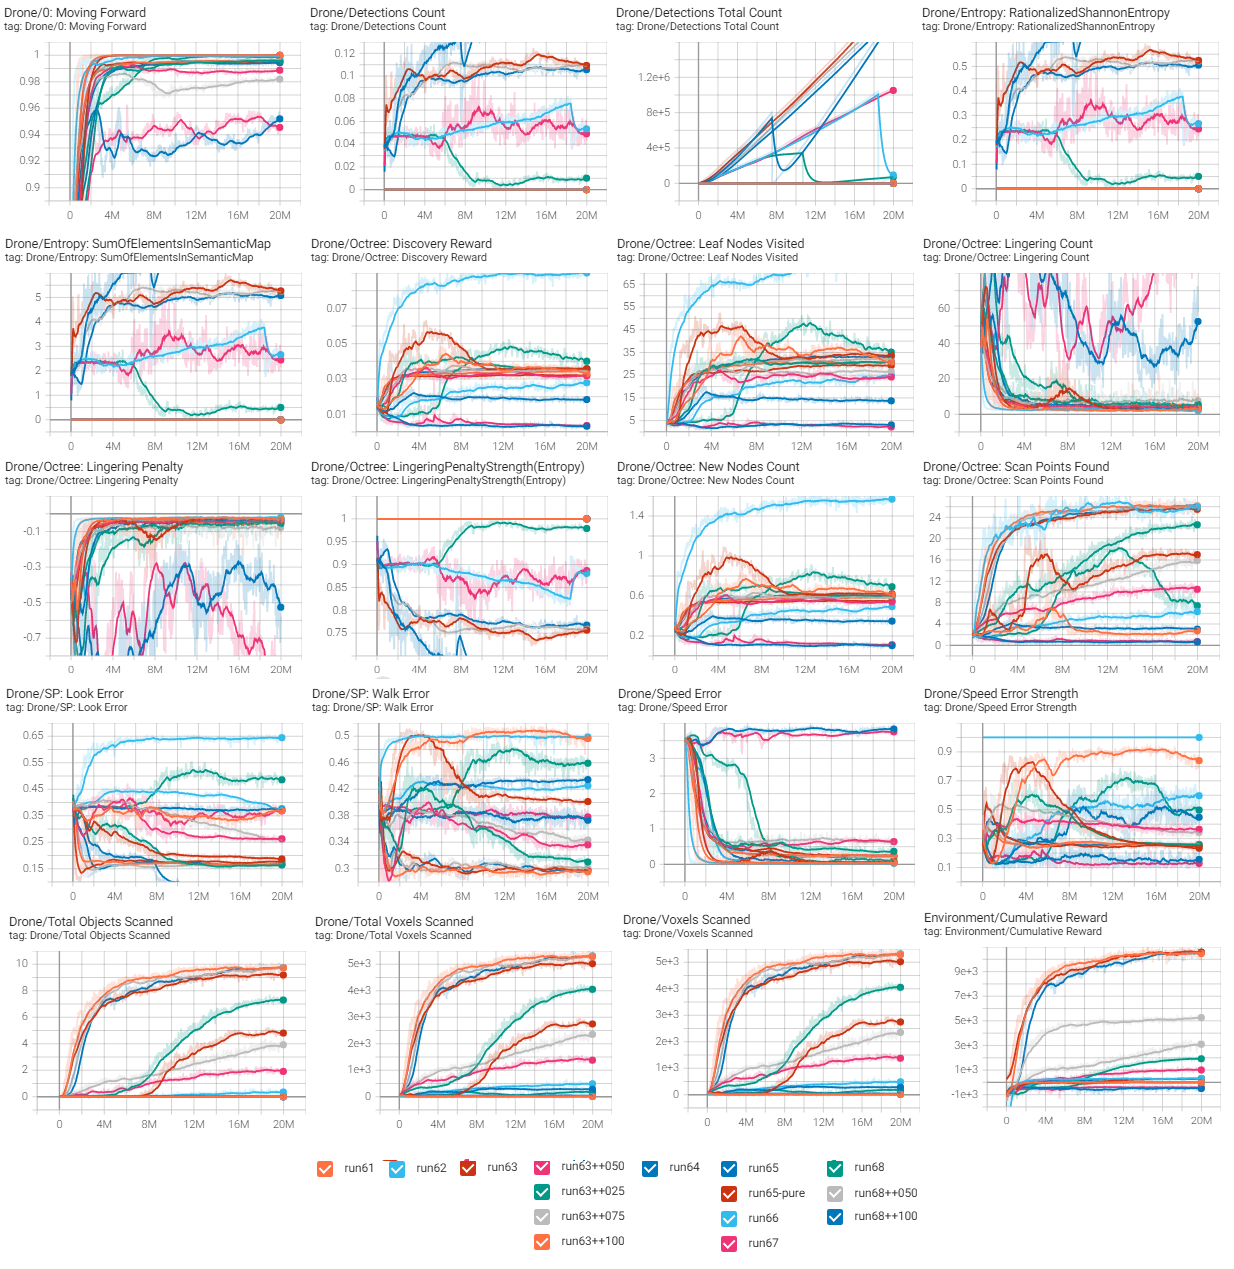
\includegraphics[width=1\textwidth]{images/results_baseAgent.png}
        \caption{Small environment result (size: 32 $m^2$) .
        }
        \label{fig:results-small-env-performances}
\end{figure}

